\chapter{Introduction}

Agile software development's ideas and principles go back to the early 1960s and have been laid down in 2001 with the Agile Manifesto~\citep{beck2001agile}. Ever since the industry's need to adjust and respond to change quicker, in order to deliver higher business value, did not lose importance. Partially promising these results, agile is geared towards being applied within small, loosely coupled teams, all working mostly independently~\citep{stober2009agile}. Embracing and transitioning towards any new work environment embodies barriers on a people and organisational level, both in their scale of magnitude being company dependent~\citep{schiel2009enterprise}. The general acceptance of agile grows towards 84\% but it is mostly applied within companies of intermediate size~\citep{7thagilesur}. This is where bigger corporations tend to be confronted with a larger set of issues brought about by more defined practices and processes and a strict and well-defined organisational structure~\citep{schiel2009enterprise}. These structures are not always fully static and are often subject to change but still can not be fully left behind in favour of agile as they are motivated by a need for coordination within a big scale.

Research has largely focused on general advice towards transformations from waterfall to agile development models. Nevertheless, it has been less concerned with belated integration difficulties that follow after the adoption of agile methods~\citep{ivari2011orgagile}. The academia mostly paid attention to communication within~\acp{XFT}~\citep{stray2012investigatingdailyteam, kauffeld2011meetingsmatter, pikkarainen2008impactagilecommunication} and the productivity of agile methodologies in general~\citep{badampudi2013proddelay, leffingwell2007scalelargecorps}. To the authors best knowledge, there is a lack of literature investigating~\acp{XFT} and their communication with other units in large organisations, its associated challenges and their impact on productivity. 
This area is worthy of attention as agile's popularity increases and gains attention from organisations of different context and size.

The thesis investigates and questions agile's compatibility with large organisations' structures with a focus on problematic aspects of communication, its paths and intersections and the resulting information flow with potential blockages. Hence, research questions focus on challenges associated with information (RQ1) and communication (RQ2) and relate their interplay to the organisation's scale. Finally, it discovers the organisation's influence on the work of its~\acp{XFT} from the perspectives of productivity determinants (RQ3). To this end, the thesis reports on a case study conducted over a four month period in cooperation with one of the software development organisations at Ericsson AB --- \ac{PDU LMR}. As performance fluctuations and discrepancies within the organisation became visible over the course of the adoption of agile methodologies, it seems that especially issues around communication and information hinder taking full advantage of agile software development.

The study employs both quantitative and qualitative methods in form of daily surveys and semi-structured interviews respectively. Week long daily surveys with the two groups of participants of 20 people in total highlight the paths and intensities of different types of communication. A qualitative part of the research addresses issues of communication and information by obtaining personal opinions and experiences of a subset of the survey's participants with 13 employees of different roles.

The results, as illustrated without greater detail in Figure~\ref{fig:intro-theming}, give an explanation of how challenges within communication and information relate to the benefits of their overcoming and which potential improvements are needed to yield associated benefits. Ultimately, it raises awareness and understanding towards multiple trade-offs to be made by the organisation within \ac{XFT} empowerment, XFT workflow, and organisational environment to impact their productivity.

\begin{figure}[h!]
  \centering
  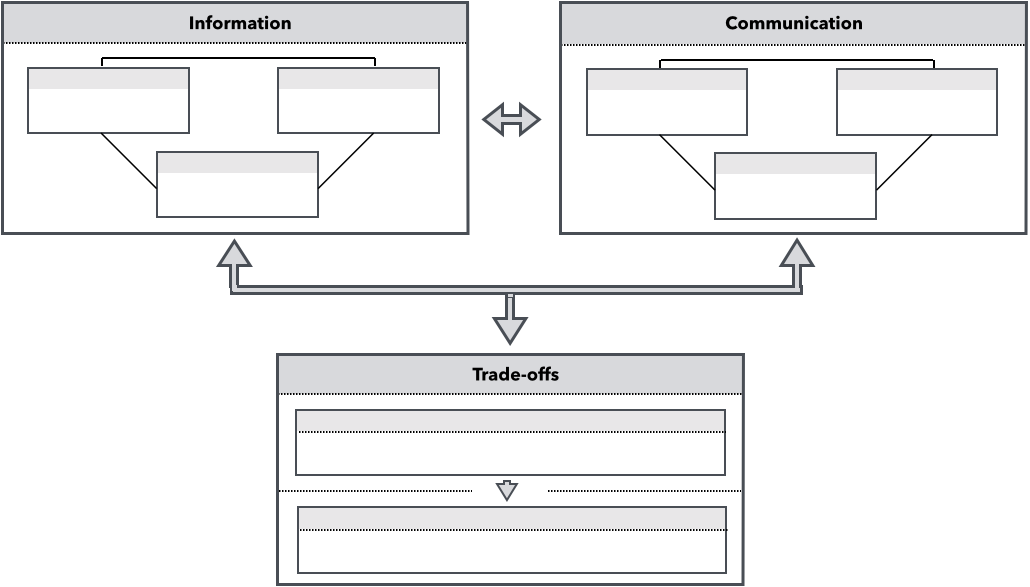
\includegraphics[width=0.90\textwidth]{figures/intro-theming-diagram.png}
  \caption{Overview of relationship between information, communication and trade-offs}
  \label{fig:intro-theming}
\end{figure}

The remainder of this thesis is structured as follows: Section~\ref{chap:related-work} presents related work in the area of agile principles, agile at scale, and agile coordination and communication. Section~\ref{chap:background} lays a foundation regarding theoretical concepts such as communication and information, heat maps and social networks. Section~\ref{chap:research-methodology} describes the case study's research methodology from its context to data collection and analysis and elaborates on threats to validity. Section~\ref{chap:findings} presents findings which are discussed and interpreted in Section~\ref{chap:discussion}. Section~\ref{chap:conclusions} concludes the thesis work and gives recommendations for further research.
